%xelatex -shell-escape -output-directory=bin ergasia.tex
\documentclass{assignment}

\university{Πανεπιστήμιο Πειραιώς}{Πα.Πει.}
\school{Τμήμα Πληροφορικής}{Π.Μ.Σ. "Πληροφορική"}
\department{Πρόγραμμα Μεταπτυχιακών Σπουδών «Πληροφορική»}{}
%\cover{images/cover.jpg}{http://www.cyberciti.biz/faq/grub-boot-into-single-user-mode/}

\title{Τεχνολογίες Διαδικτύου \\ 4η Εργασία}
%\projectlevel{Εργαστήριο Λειτουργικά Συστήματα}
%\lesson{Λειτουργικά Συστήματα}{1}
\date{Αθήνα, 2014}

\author{Αναγνωστόπουλος Βασίλης - Θάνος, Κατσής Γεώργιος}
%\register{ΜΠΠΛ13002}{1}

%\exercauthor{Αναγνωστόπουλος Βασίλης - Θάνος}{06107083}{9}

%\advisor{Τσακίρη Μαρία, Αναπληρώτρια Καθηγήτρια Ε.Μ.Π.}

\begin{document}

\maketitle
% Να σκεφτώ τί αλλαγές θέλω να κάνω με τις αριθμήσεις και άμα θέλω να κάνω.
% Να σκεφτώ να τις ενσωματώσω και στο assignment.cls

\setcounter{page}{1} 
\pagenumbering{roman}

\pagestyle{plain}
\tableofcontents
\newpage


%\pagestyle{headings}
\pagestyle{fancy}
\setcounter{page}{1} 
\pagenumbering{arabic}

\begin{Assignment}%[Ερώτημα]
\AssignmentTitle{ % 
Δημιουργήστε μία ιστοσελίδα.

Παρατηρήσεις:

\begin{itemize}
\item Ακολουθήστε τους κανόνες σύνταξης της HTML5.
\item Μαζί με τον πηγαίο κώδικα θα παραδώσετε και λεπτομερέστατο έγγραφο όπου θα
εξηγείτε πως δημιουργήσατε οτιδήποτε εμφανίζετε στην ιστοσελίδα σας. 
\end{itemize}
}

Ο κώδικας που υλοποιεί την σελίδα φαίνεται παρακάτω.

\inputminted[linenos,tabsize=2]{html}{../../index.html}
\captionof{listing}{Ο κώδικας της σελίδας \label{html_code}}

\inputminted[linenos,tabsize=2]{css}{../../theme.css}
\captionof{listing}{Ο κώδικας css της σελίδας \label{css_code}}

\inputminted[linenos,tabsize=2]{js}{../../javascript.js}
\captionof{listing}{Ο κώδικας javascript της σελίδας \label{javascript_code}}

Ακόμα η σελίδα έχει "ανέβει" στην διεύθυνση \url{http://tme121.anagno.me}
και ο κώδικας της βρίσκεται στο \url{https://github.com/giokats/Texnologies_Diadiktiou}
\end{Assignment}

Τέλος ο κώδικας της σελίδας ελέγχθηκε χρησιμοποιώντας το \url{http://validator.w3.org} (εικόνα 
\ref{fig:date})

\begin{figure}
\begin{center}
\resizebox*{!}{8.5cm}{
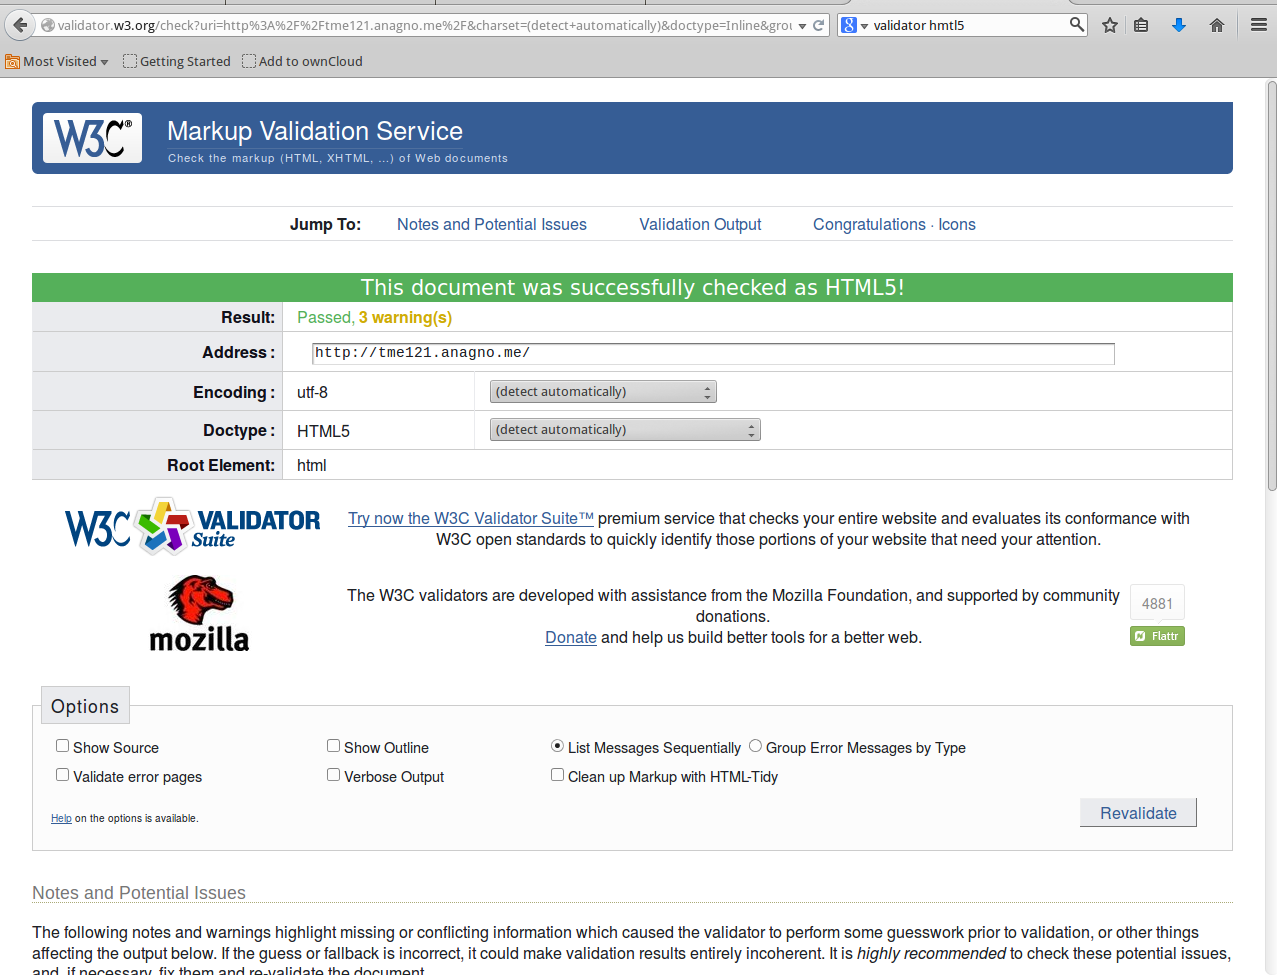
\includegraphics{images/validator.png}}
\caption{Screenshot από το \url{http://validator.w3.org} }
\label{fig:date}
\end{center}
\end{figure}

\begin{figure}
\begin{center}
\resizebox*{!}{8.5cm}{
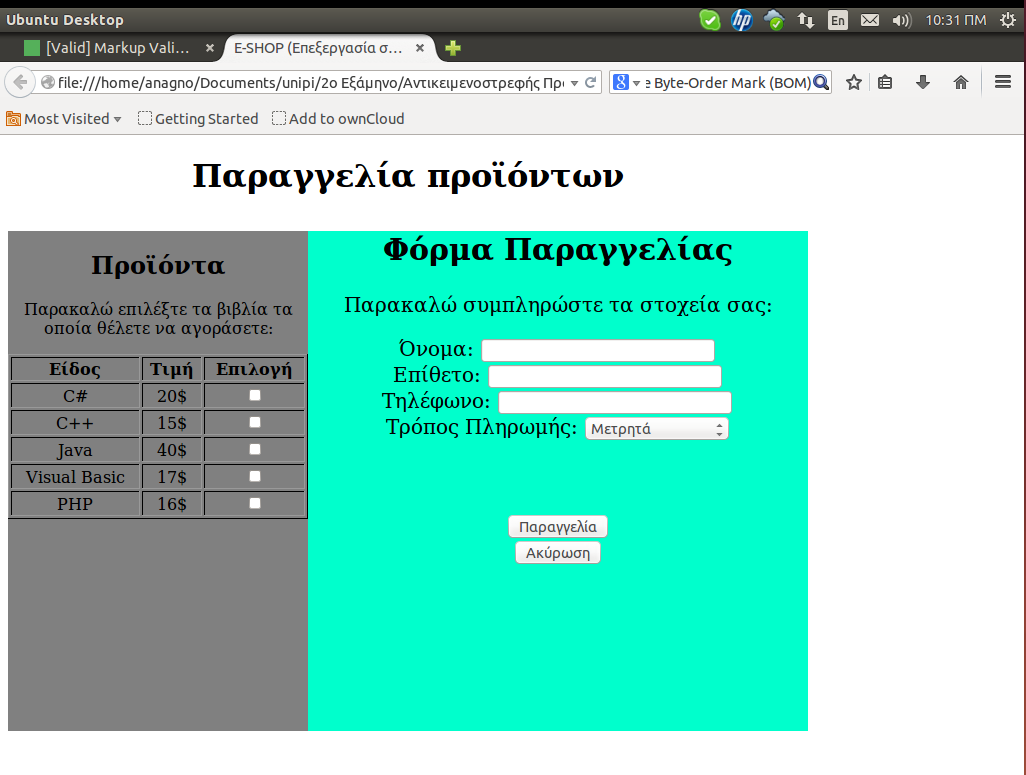
\includegraphics{images/site.png}}
\caption{Screenshot από την ιστοσελίδα χρησιμοποιώντας τον \en{firefox} }
\label{fig:site}
\end{center}
\end{figure}

\begin{figure}
\begin{center}
\resizebox*{!}{8.5cm}{
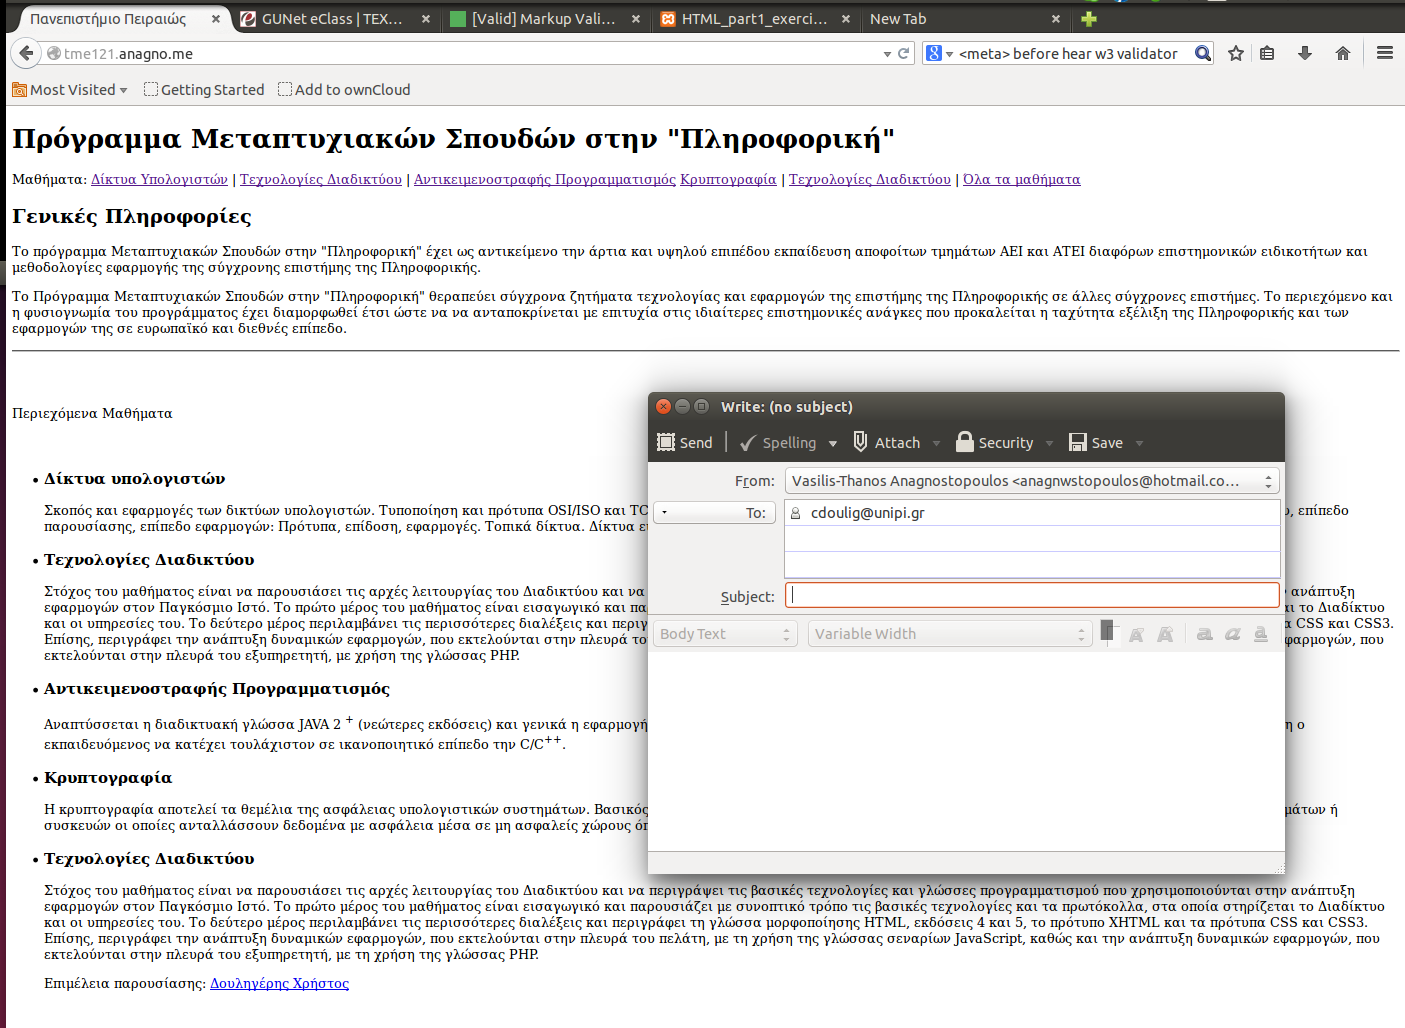
\includegraphics{images/mail.png}}
\caption{Screenshot έχοντας πατήσει το μαιλ χρησιμοποιώντας το \en{thunderbird} }
\label{fig:mail}
\end{center}
\end{figure}
\newpage

%\phantomsection \label{Βιβλιογραφία}
%\addcontentsline{toc}{section}{Βιβλιογραφία}
%\mtcaddchapter[Βιβλιογραφία] % Λόγω του minitoc
%\bibliographystyle{plain}
%\bibliography{references}


\end{document}

1
